\chapter{Background on Deep Learning}

In the task of image classification, traditional machine learning algorithms required hand-engineered features, like filters and descriptors, which were meant to extract information from the images to be used as an input for algorithms. These algorithms would then be trained to find patterns in these features capable of distinguishing between different classes.

Neural networks, on the other hand, have the advantage of being able to learn these features directly from the data, which makes the process of feature engineering a lot simpler and achieves better results in most cases. Furthermore, the recent advances in deep neural networks have taken these capabilities to a new level. They not only win most of the competitions in the field but also achieve state of the art results in a wide range of real applications. One type of network that is responsible for these results is the Convolutional Neural Network (CNN) \citep{Lecun1998}.

\section{Convolutional Neural Networks}

Convolutional neural networks are similar to traditional neural networks. They both have an input layer which receives the data, followed by hidden layers with numerous neurons with weights and biases capable of learning the characteristics of the data, and a fully connected output layer at the end which is responsible for classification. The main difference is that CNNs assume the input has some spatial relationship, which is a pattern present in images. Thus, knowledge of where pixels are located in reference to each other is preserved. CNNs are capable of extracting and capturing patterns from the images that would not have been possible if we used traditional networks. To extract these features, the networks uses two primary operations: convolution and pooling.

Convolutions are linear mathematical operations that act as learnable filters (also called kernels) to capture patterns in the images. These filters are usually small in terms of dimension, typically 3x3 or 5x5 matrices. Each one of them convolves across the width and height of the input image and compute dot products with the pixels of the image, producing an activation map out of it. These activation maps, once learned, are able to detect features in the images, such as edges, corners, or color shifts. 

\begin{figure}[h!tp]
    \centering
    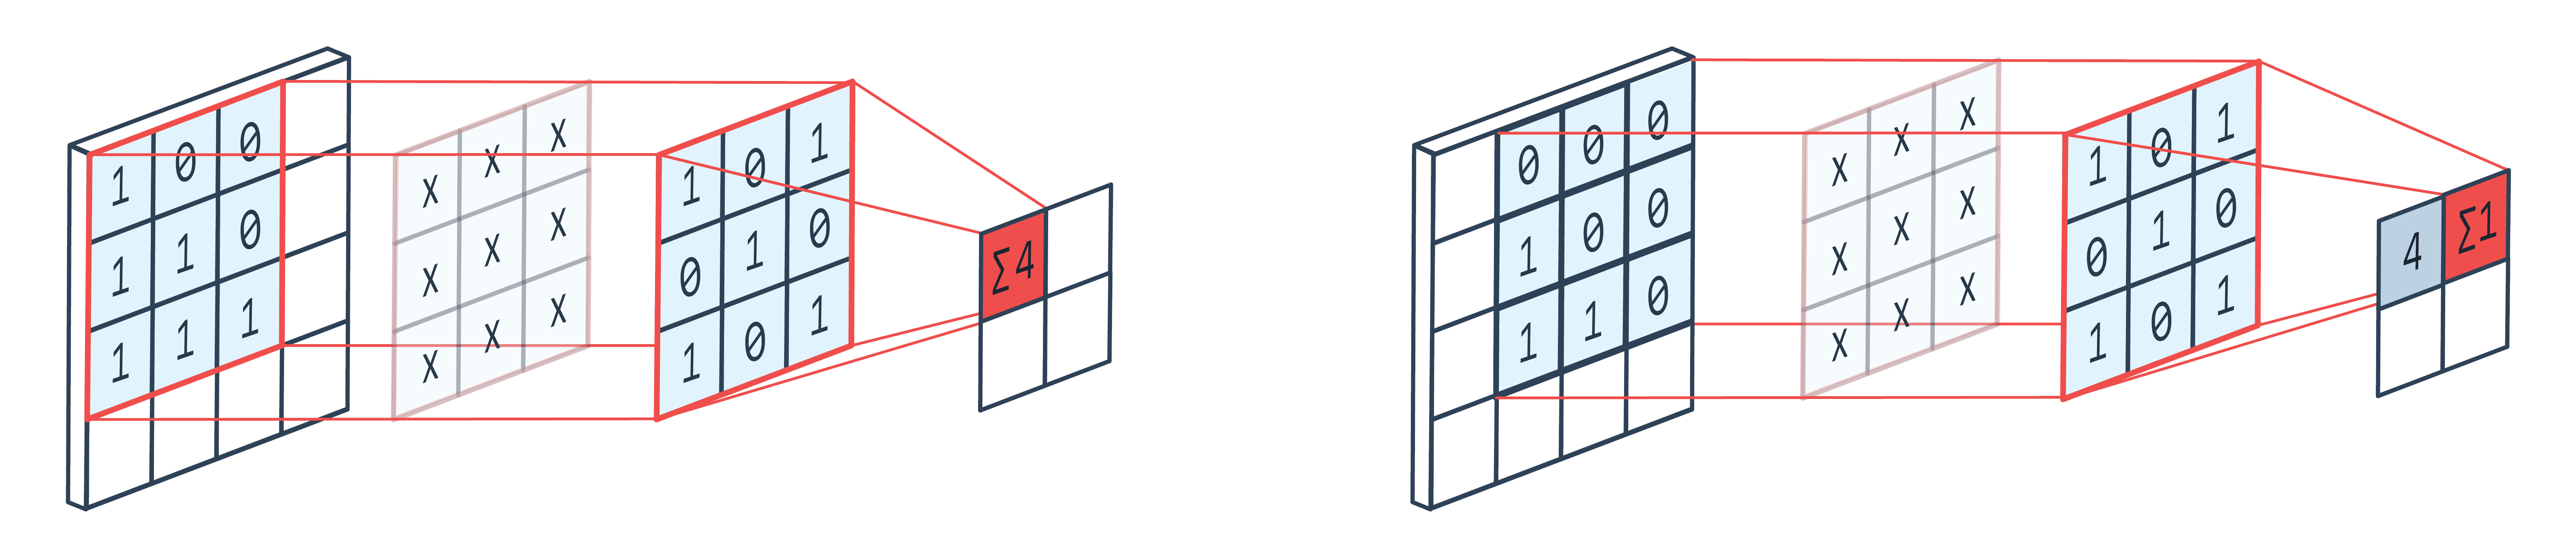
\includegraphics[width=.89\textwidth]{imgs/chap3_convolution.png}
    \caption[The convolution operation.]{The convolution operation. Figure extracted from the Peltarion website\footnotemark.}
    \label{fig:convolution}
\end{figure}

\footnotetext{\url{https://bit.ly/38bR3uK}}

Pooling is another mathematical operation responsible for reducing the spatial size of the convolved feature. These series of transformations reduce the dimensionality of the data and makes it possible to process images of high resolution. The most common cases of pooling are average pooling and max pooling, which are illustrated on Figure \ref{fig:pooling}.

\begin{figure}[h!tp]
\centering
\begin{subfigure}{.45\textwidth}
  \centering
  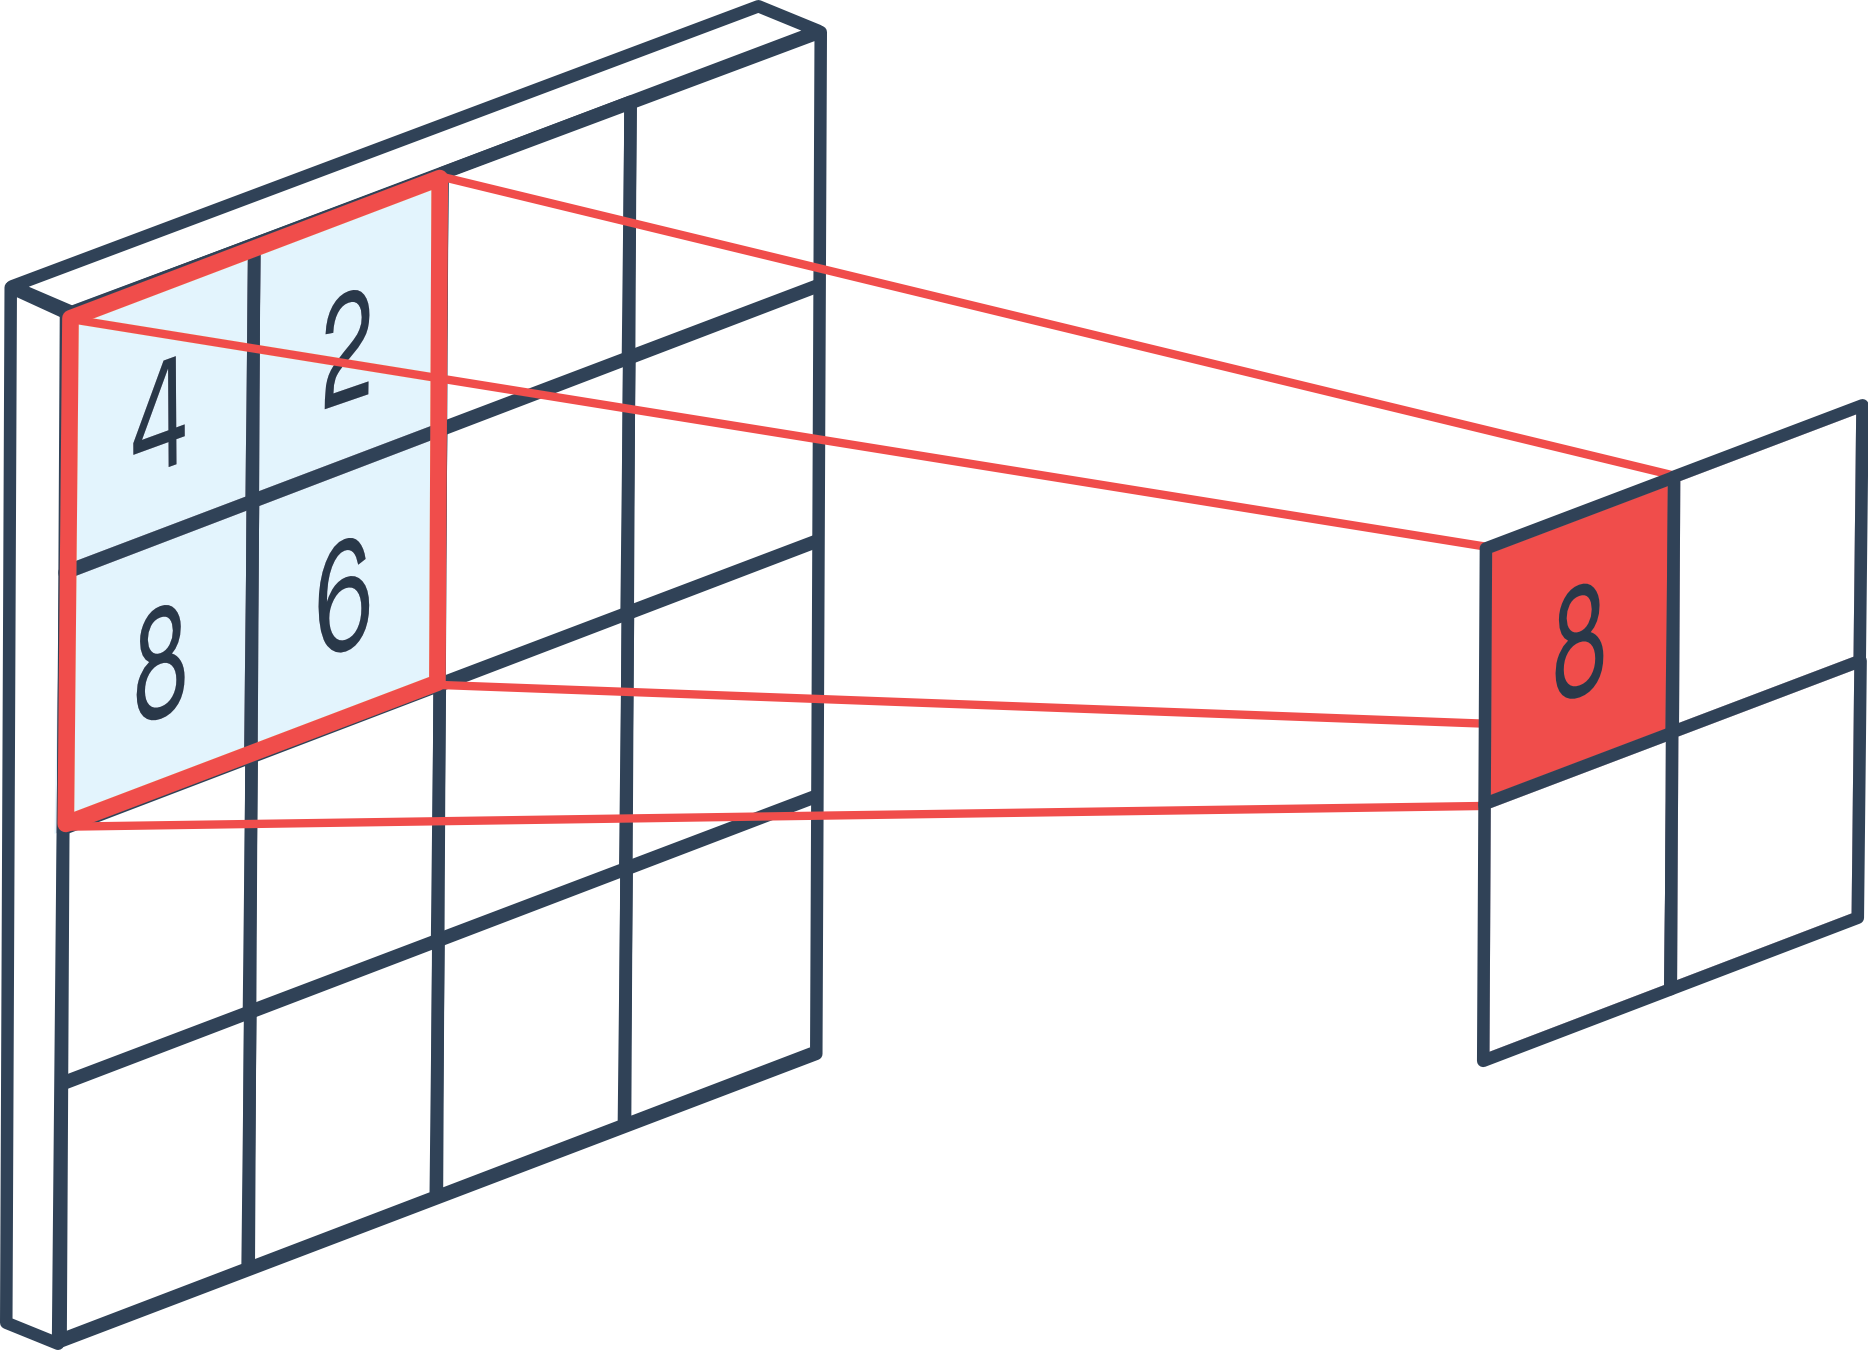
\includegraphics[width=.5\linewidth]{imgs/chap3_max_pooling.png}
  \caption{Average Pooling}
  \label{fig:sub1}
\end{subfigure}
\begin{subfigure}{.45\textwidth}
  \centering
  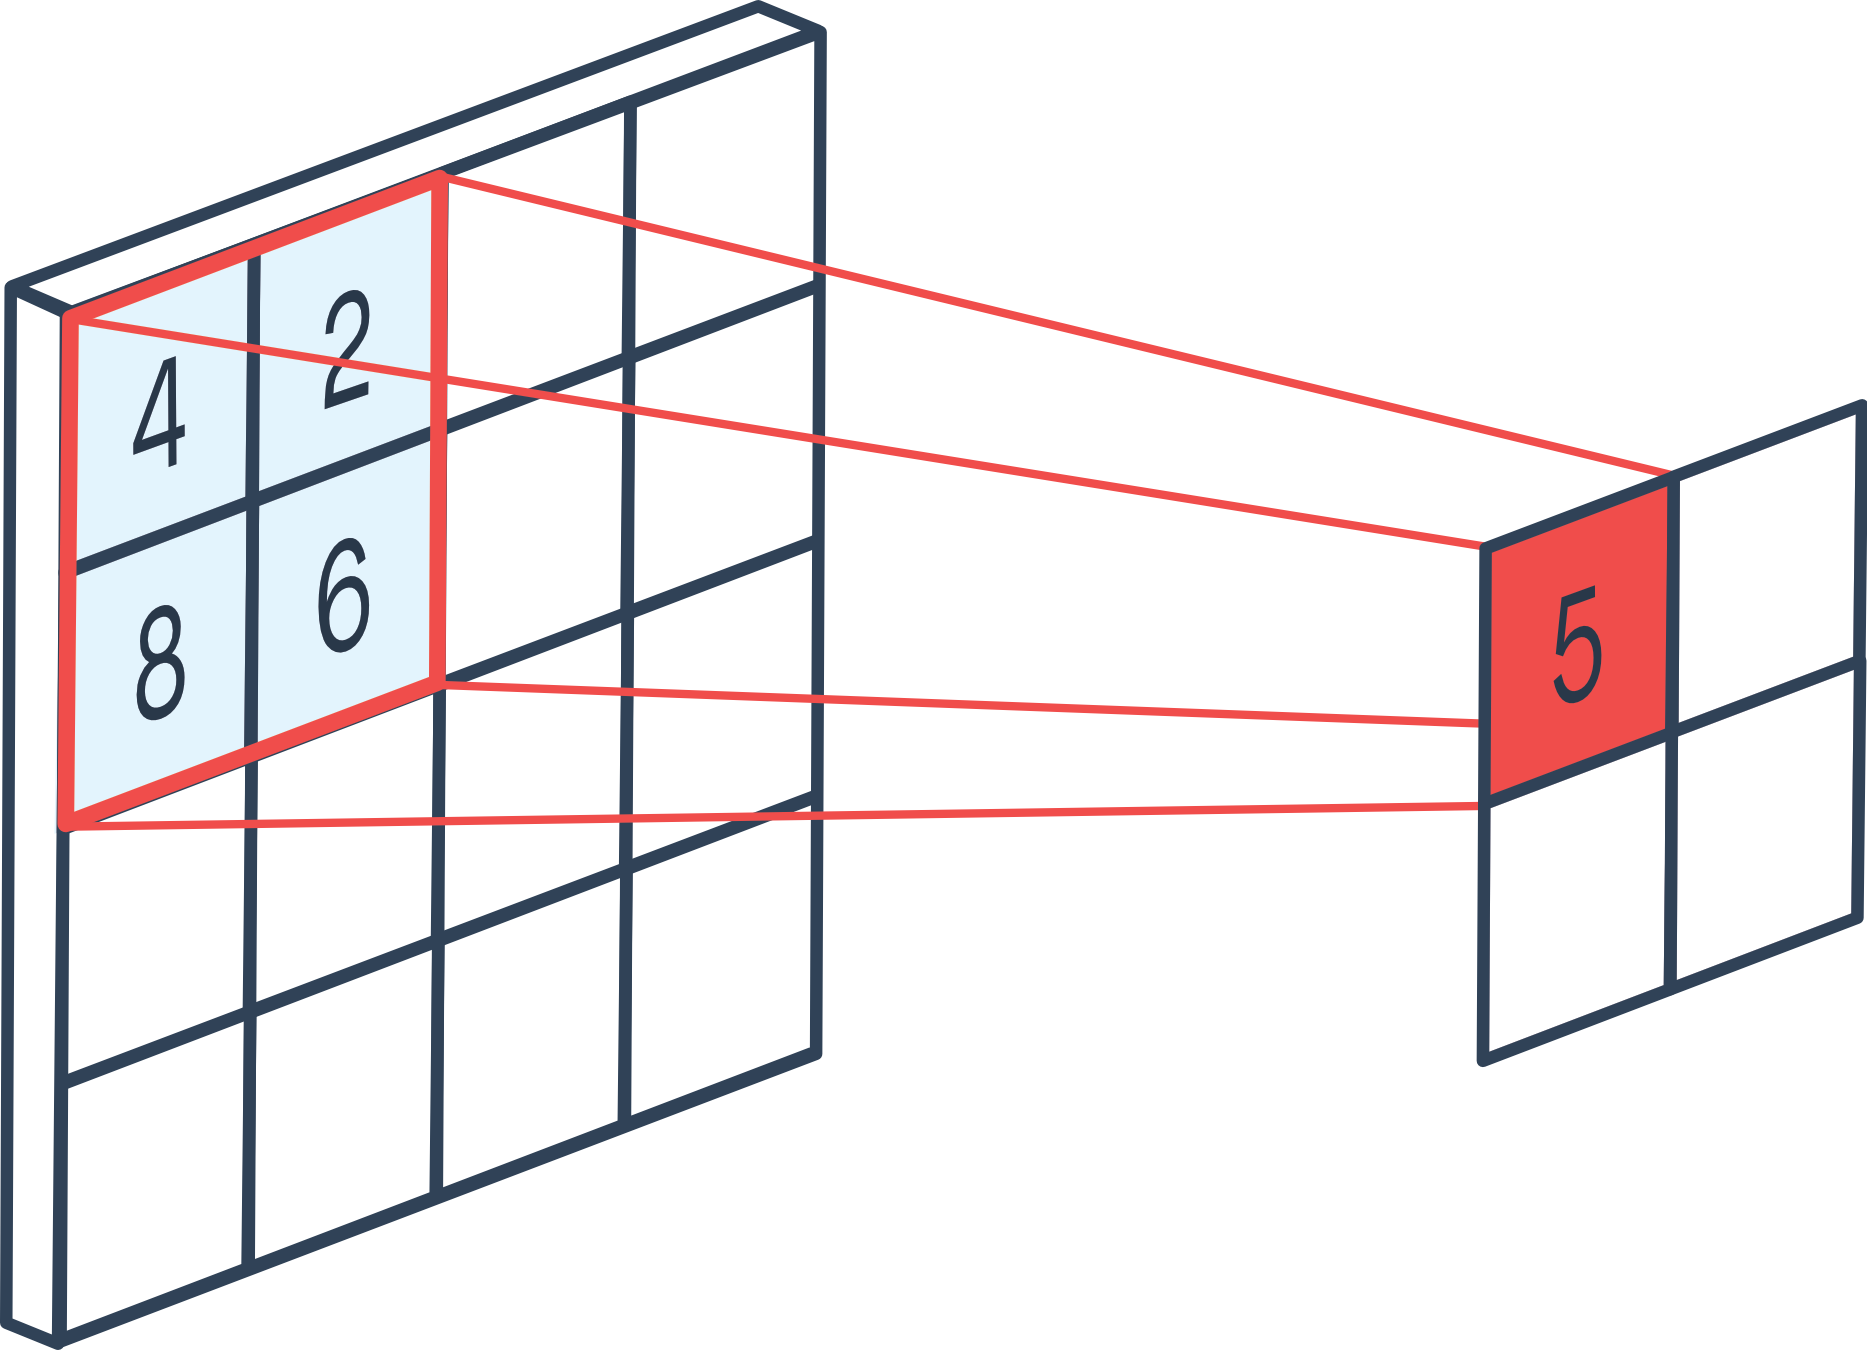
\includegraphics[width=.5\linewidth]{imgs/chap3_avg_pooling.png}
  \caption{Max Pooling}
  \label{fig:sub2}
\end{subfigure}
\caption[Common pooling types.]{Common pooling types. Figure extracted from the Peltarion website\footnotemark.}
\label{fig:pooling}
\end{figure}

\footnotetext{\url{https://bit.ly/2Pzpkxq}}

As multiple convolutional and pooling layers get stacked, the network becomes able to detect more complex patterns that are composed of multiple inputs of different feature extractors in the first layers. By turning this activation maps back into images, we are able to see what kinds of features they are detecting, as demonstrated by \citep{ZeilerF14}.

\section{Transfer Learning}

Transfer Learning is a technique commonly used in machine learning when a learning model that was originally developed for one task is then reused on a second related task. It comes from the assumption that what has been learned in one setting can be used to improve optimization in another setting. The idea behind is inspired by human behavior, as sometimes we can use expertise in solving one problem to solve a new one.

Another motivation behind using transfer learning comes from the high computational cost necessary to train large deep neural networks for image classification. Since the number of parameters present in a CNN is very high, it requires a large amount of training data to tune the network for making precise predictions.

As an example, a commonly used dataset in the field for pre-training networks is a subset of ImageNet \citep{DengDSLL009}, which contains 1.2 million images and has 1000 labeled categories for classification. Even with today's computational power, it still requires a significant amount of hours to be trained.

In this scenario, using transfer learning trough pre-trained networks arises as a solution. In this process, the weights and biases from a network trained in another task, are reused to train a new similar task.

Another reason for using transfer learning comes from the cases where we do not have enough data to train a CNN. \cite{CelonaBB19} highlights this is especially true in the medical field, as the acquisition costs are elevated, and it also involves a complicated set-up for photographing, which makes it very common to have little annotated data.

\section{Data Augmentation}

Another solution that handles small datasets is data augmentation. It consists of applying transformations, such as geometric and color augmentations, for generating alternative images that derive from the original dataset.

For each input image in the dataset, a new image is generated that can be zoomed, shifted, mirrored, rotated, distorted, or have changes in its color, brightness, contrast. Hence, this technique increases the amount of data available for input. 

Having a large dataset is crucial for the performance of the deep learning models, but instead of starting with a large dataset of images, a more common scenario is to have a small amount of data available from the specific domain of research. This usually happens due to the high cost of collecting data, be it in terms of human labor or monetary resources. As mentioned in the previous section, this is mainly the case in the medical field. 

Another problem of small datasets is that problems trained on them are often over-fitted to the specific data available, which means they lack the power of generalization, as the dataset is not representative of the real world. In these cases, as discussed by \cite{abs-1712-04621}, data augmentation can act as a regularizer for preventing over-fitting and also improve performance in imbalanced class problems.
